\documentclass{article}
\newenvironment{standalone}{\begin{preview}}{\end{preview}}
\usepackage{../includes}

\begin{document}
\begin{standalone}

\section{Desarrollo de la aplicación}

\subsection{Configuración}

\subsubsection{Configuración de Unity}

Para el correcto funcionamiento del entorno de desarrollo de la aplicación del presente proyecto, se deberá seguir las siguientes instrucciones para instalar y configurar Unity y los paquetes y plugins necesarios.

\href{https://unity3d.com/get-unity/download}{Descargar} e instalar Unity Hub.
Al iniciar Unity Hub, seleccionar la versión de Unity 2019.4.22f para descargar e instalar.
Durante la instalación, incluir el módulo \textit{Android Build Support} y, dentro de éste, asegurarse de incluir \textit{Android SDK \& NDK tools} y \textit{OpenJDK}.
Aunque el desarrollo es para Android, incluir también el módulo \textit{iOS Build Support} para evitar errores en ARCore.

\href{https://github.com/google-ar/arcore-unity-sdk/releases}{Descargar} el paquete de ARCore SDK para Unity v1.23.0.
Seguir la guía \href{https://developers.google.com/ar/develop/unity/quickstart-android?hl=en}{\textit{Quickstart for Android}} para instalarlo y configurarlo.
En resumen, descargar e instalar Android Studio con Android SDK 7.0 o superior.
Crear un nuevo proyecto 3D en Unity.
Ir a \textit{Windows >\ Package Manager} y descargar los paquetes \textit{Multiplayer HLAPI} y \textit{XR Legacy Input Helpers}.
Ir a \textit{Assets >\ Import Package >\ Custom Package} y seleccionar el archivo \textit{.unitypackage} descargado previamente para importar el paquete ARCore.
Abrir el proyecto de muestra \textit{HelloAR} en \textit{Assets/GoogleARCore/Examples/HelloAR/Scenes/}.
Ir a \textit{File >\ Build Settings} y seleccionar Android como plataforma, luego hacer click en \textit{Player Settings}. Allí, configurar, dentro de \textit{Other Settings}, \textit{Minimum API Level} en 24, \textit{Scripting Backend} en IL2CPP, \textit{Target Architectures} en ARM64 y, dentro de \textit{XR Settings}, habilitar la opción \textit{ARCore Supported}.

Conectar el teléfono a la computadora y, estando en \textit{Build Settings}, hacer click en \textit{Build and Run}. Se genera un archivo \textit{.apk} que se instala y ejecuta en el teléfono.
Luego de comprobar que la aplicación de prueba \textit{HelloAR} funciona correctamente, se la puede utilizar de plantilla para el desarrollo de la presente aplicación.

Descargar e instalar el plugin \textit{Android \& Microcontrollers / Bluetooth} desde la \href{https://assetstore.unity.com/packages/tools/input-management/android-microcontrollers-bluetooth-16467}{\textit{Unity Asset Store}}.
Este plugin necesita modificar el archivo \textit{AndroidManifest.xml} del proyecto, para eso, primero se lo debe generar en \textit{File >\ Build Settings >\ Player Settings >\ Publishing Settings} habilitando la opción \textit{Custom Main Manifest}.
Luego, ir a \textit{Tools >\ TechTweaking >\ Bluetooth Classic >\ Setup the BT Library} para iniciar la configuración automática del plugin.

\href{https://github.com/nenuadrian/qr-code-unity-3d-read-generate}{Descargar} la librería \textit{ZXing} y colocar el archivo \textit{zxing.unity.dll} en la carpeta \textit{/Plugins} del proyecto.

\subsubsection{Configuración de la Raspberry Pi}

Lo primero que se debe realizar es instalar un sistema operativo en la Raspberry Pi.
Siguiendo la guía \href{https://projects.raspberrypi.org/en/projects/raspberry-pi-setting-up}{\textit{Setting up your Raspberry Pi}} \cite{setupRPI}, descargar y ejecutar en la computadora \textit{Raspberry Pi Imager}.
Conectar una tarjeta microSD de al menos 8GB a la computadora.
En Raspberry Pi Imager, seleccionar la última versión de Raspberry Pi OS y la microSD en la que queremos instalar el sistema operativo y esperar a que finalice la descarga e instalación.

Conectar a la Raspberry Pi la tarjeta microSD, un teclado y un mouse a los puertos USB, un monitor al puerto HDMI y una fuente de alimentación de 5V 2,5A al puerto micro-USB.
Es posible también controlar la Raspberry desde la computadora por Wi-FI realizando una configuración \textit{headless} sin necesidad de teclado, mouse y monitor.
Para ello, seguir \href{https://raspberrytips.com/pi-zero-setup-without-keyboard/}{la siguiente guía} \cite{headlessRPI}.

Cualquier teléfono debe ser capaz de descubrir y conectarse a la Raspberry Pi a través de Bluetooth para descargar los datos de navegación en cualquier momento.
El tiempo en el que el dispositivo puede ser encontrado es, por defecto, tres minutos.
Se configura este tiempo de expiración a cero para que siempre pueda encontrarse \cite{bluetoothDiscoverable}.

\noindent\begin{minipage}{\linewidth}
\begin{lstlisting}
$ sudo nano /etc/bluetooth/main.conf
DiscoverableTimeout = 0
\end{lstlisting}
\end{minipage}

Se configura la Raspberry Pi para que al iniciarse, encienda el módulo Bluetooth y permita que otros dispositivos puedan encontrarla y conectarse.

\par\noindent\begin{minipage}{\linewidth}
\begin{lstlisting}
$ sudo nano /etc/rc.local
sudo bluetoothctl <<EOF
power on
discoverable on
pairable on
EOF
\end{lstlisting}
\end{minipage}

Instalar Python 3 y PyBluez ejecutando las siguientes lineas en la terminal.

\noindent\begin{minipage}{\linewidth}
\begin{lstlisting}
$ sudo apt update
$ sudo apt install python3 idle3
$ sudo apt-get install libbluetooth-dev python-dev libglib2.0-dev libboost-python-dev libboost-thread-dev
$ pip3 install pybluez
\end{lstlisting}
\end{minipage}

\subsection{Seguimiento de movimiento}

La plantilla \textit{HelloAR} \cite{helloAR} contiene los objetos necesarios para el funcionamiento de las funciones de ARCore.
\textit{ARCore Device} contiene configuraciones de la sesión de realidad aumentada, ver \cref{fig:arsession_settings}.
Se deshabilita la detección de planos ya que no se utilizará y se selecciona el modo de estimación de luz como intensidad ambiente para aplicar a los objetos de realidad aumentada, otras opciones demandan más recursos computacionales.
\textit{First Person Camera} está vinculada a la cámara trasera del teléfono y además de parámetros de cámara, también tiene asociadas configuraciones del seguimiento de movimiento, ver \cref{fig:first_person_camera_settings}.
Principalmente, se puede seleccionar seguimiento de posición solamente o posición y rotación.
Seleccionar esta última opción, ya que si bien el seguimiento de rotación tiene un impacto negativo en la precisión del seguimiento de posición, es necesario para la integración de elementos de realidad aumentada.

\begin{figure}[ht!]
  \centering
  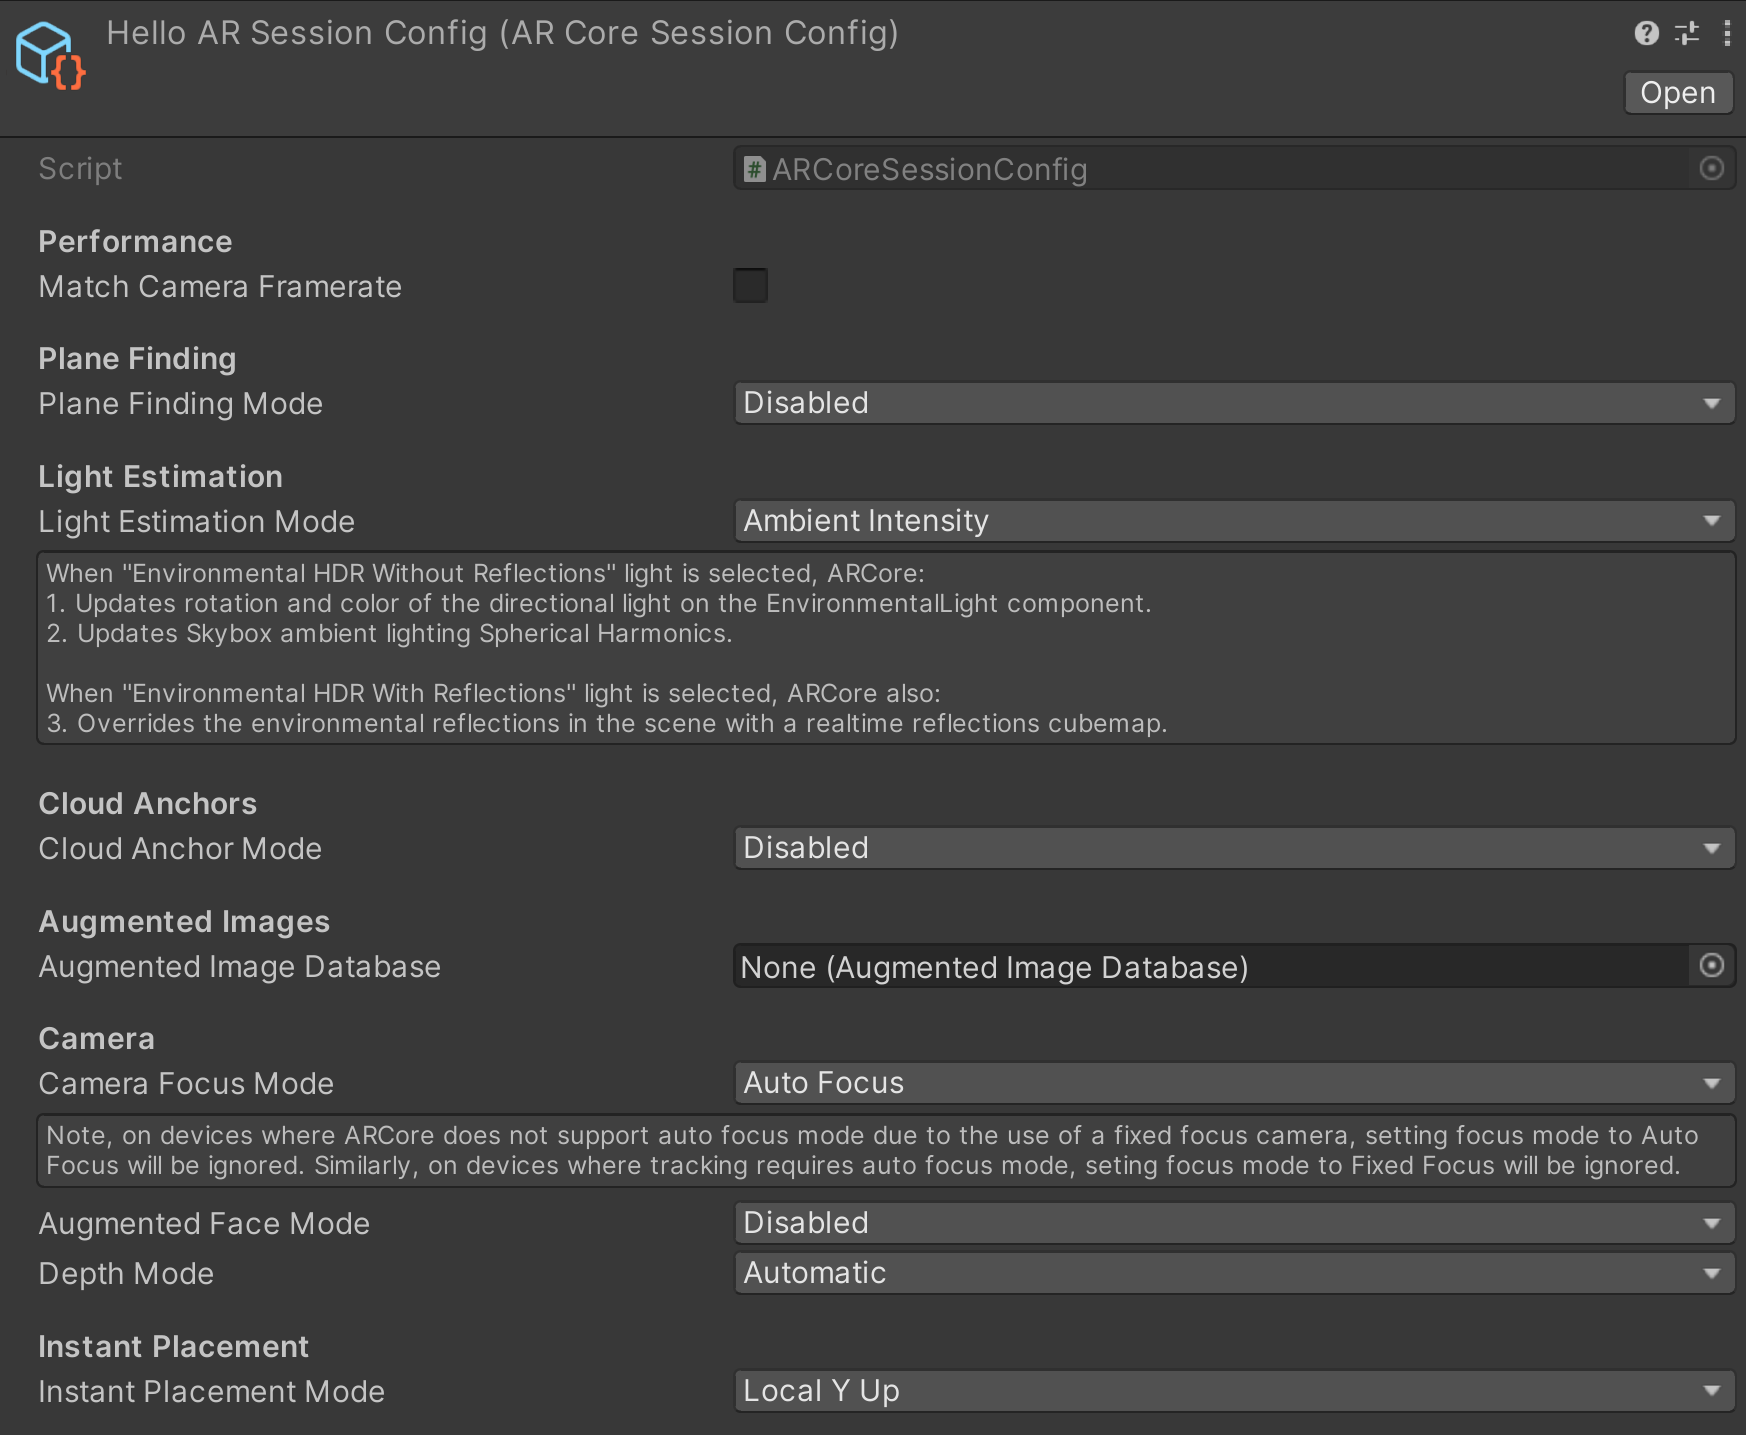
\includegraphics[width=0.65\linewidth, keepaspectratio]{arsession_settings}
  \caption{Configuración de la sesión de realidad aumentada.}
  \label{fig:arsession_settings}
\end{figure}

\begin{figure}[ht!]
  \centering
  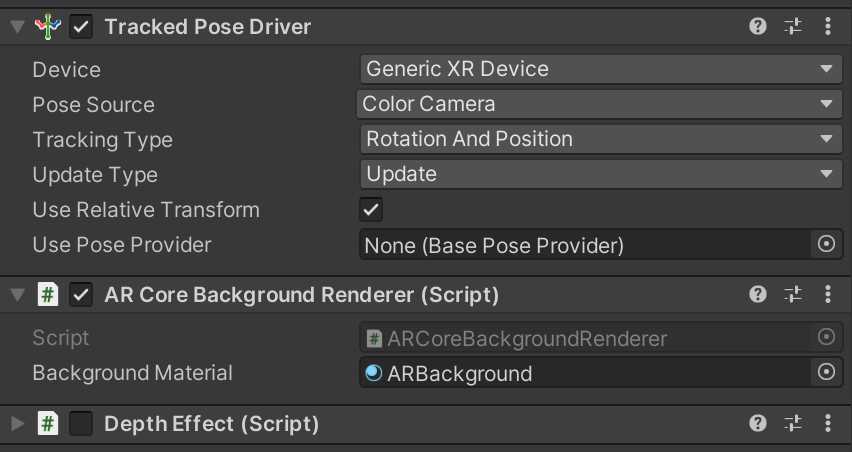
\includegraphics[width=0.65\linewidth, keepaspectratio]{first_person_camera_settings}
  \caption{Configuración de la cámara en primera persona.}
  \label{fig:first_person_camera_settings}
\end{figure}

Se crea el mapa del lugar a navegar en SolidWorks para obtener un archivo de geometría 3D a escala \textit{.obj} como se ve en la \cref{fig:mapa_solidworks}.
Este archivo se coloca en la carpeta \textit{/Prefabs} del proyecto y se inserta en la escena del proyecto.
Asegurarse de que el mapa esté a escala 1:1, es decir que un metro en la vida real tiene que equivaler a 1 unidad de Unity.
Esto puede lograrse, como se ve en la \cref{fig:escala_mapa}, con los assets de regla horizontal y vertical de \textit{zzz Ruler} que pueden descargarse desde la \href{https://assetstore.unity.com/packages/tools/utilities/zz-ruler-365}{\textit{Unity Asset Store}}

\begin{figure}[ht!]
  \centering
  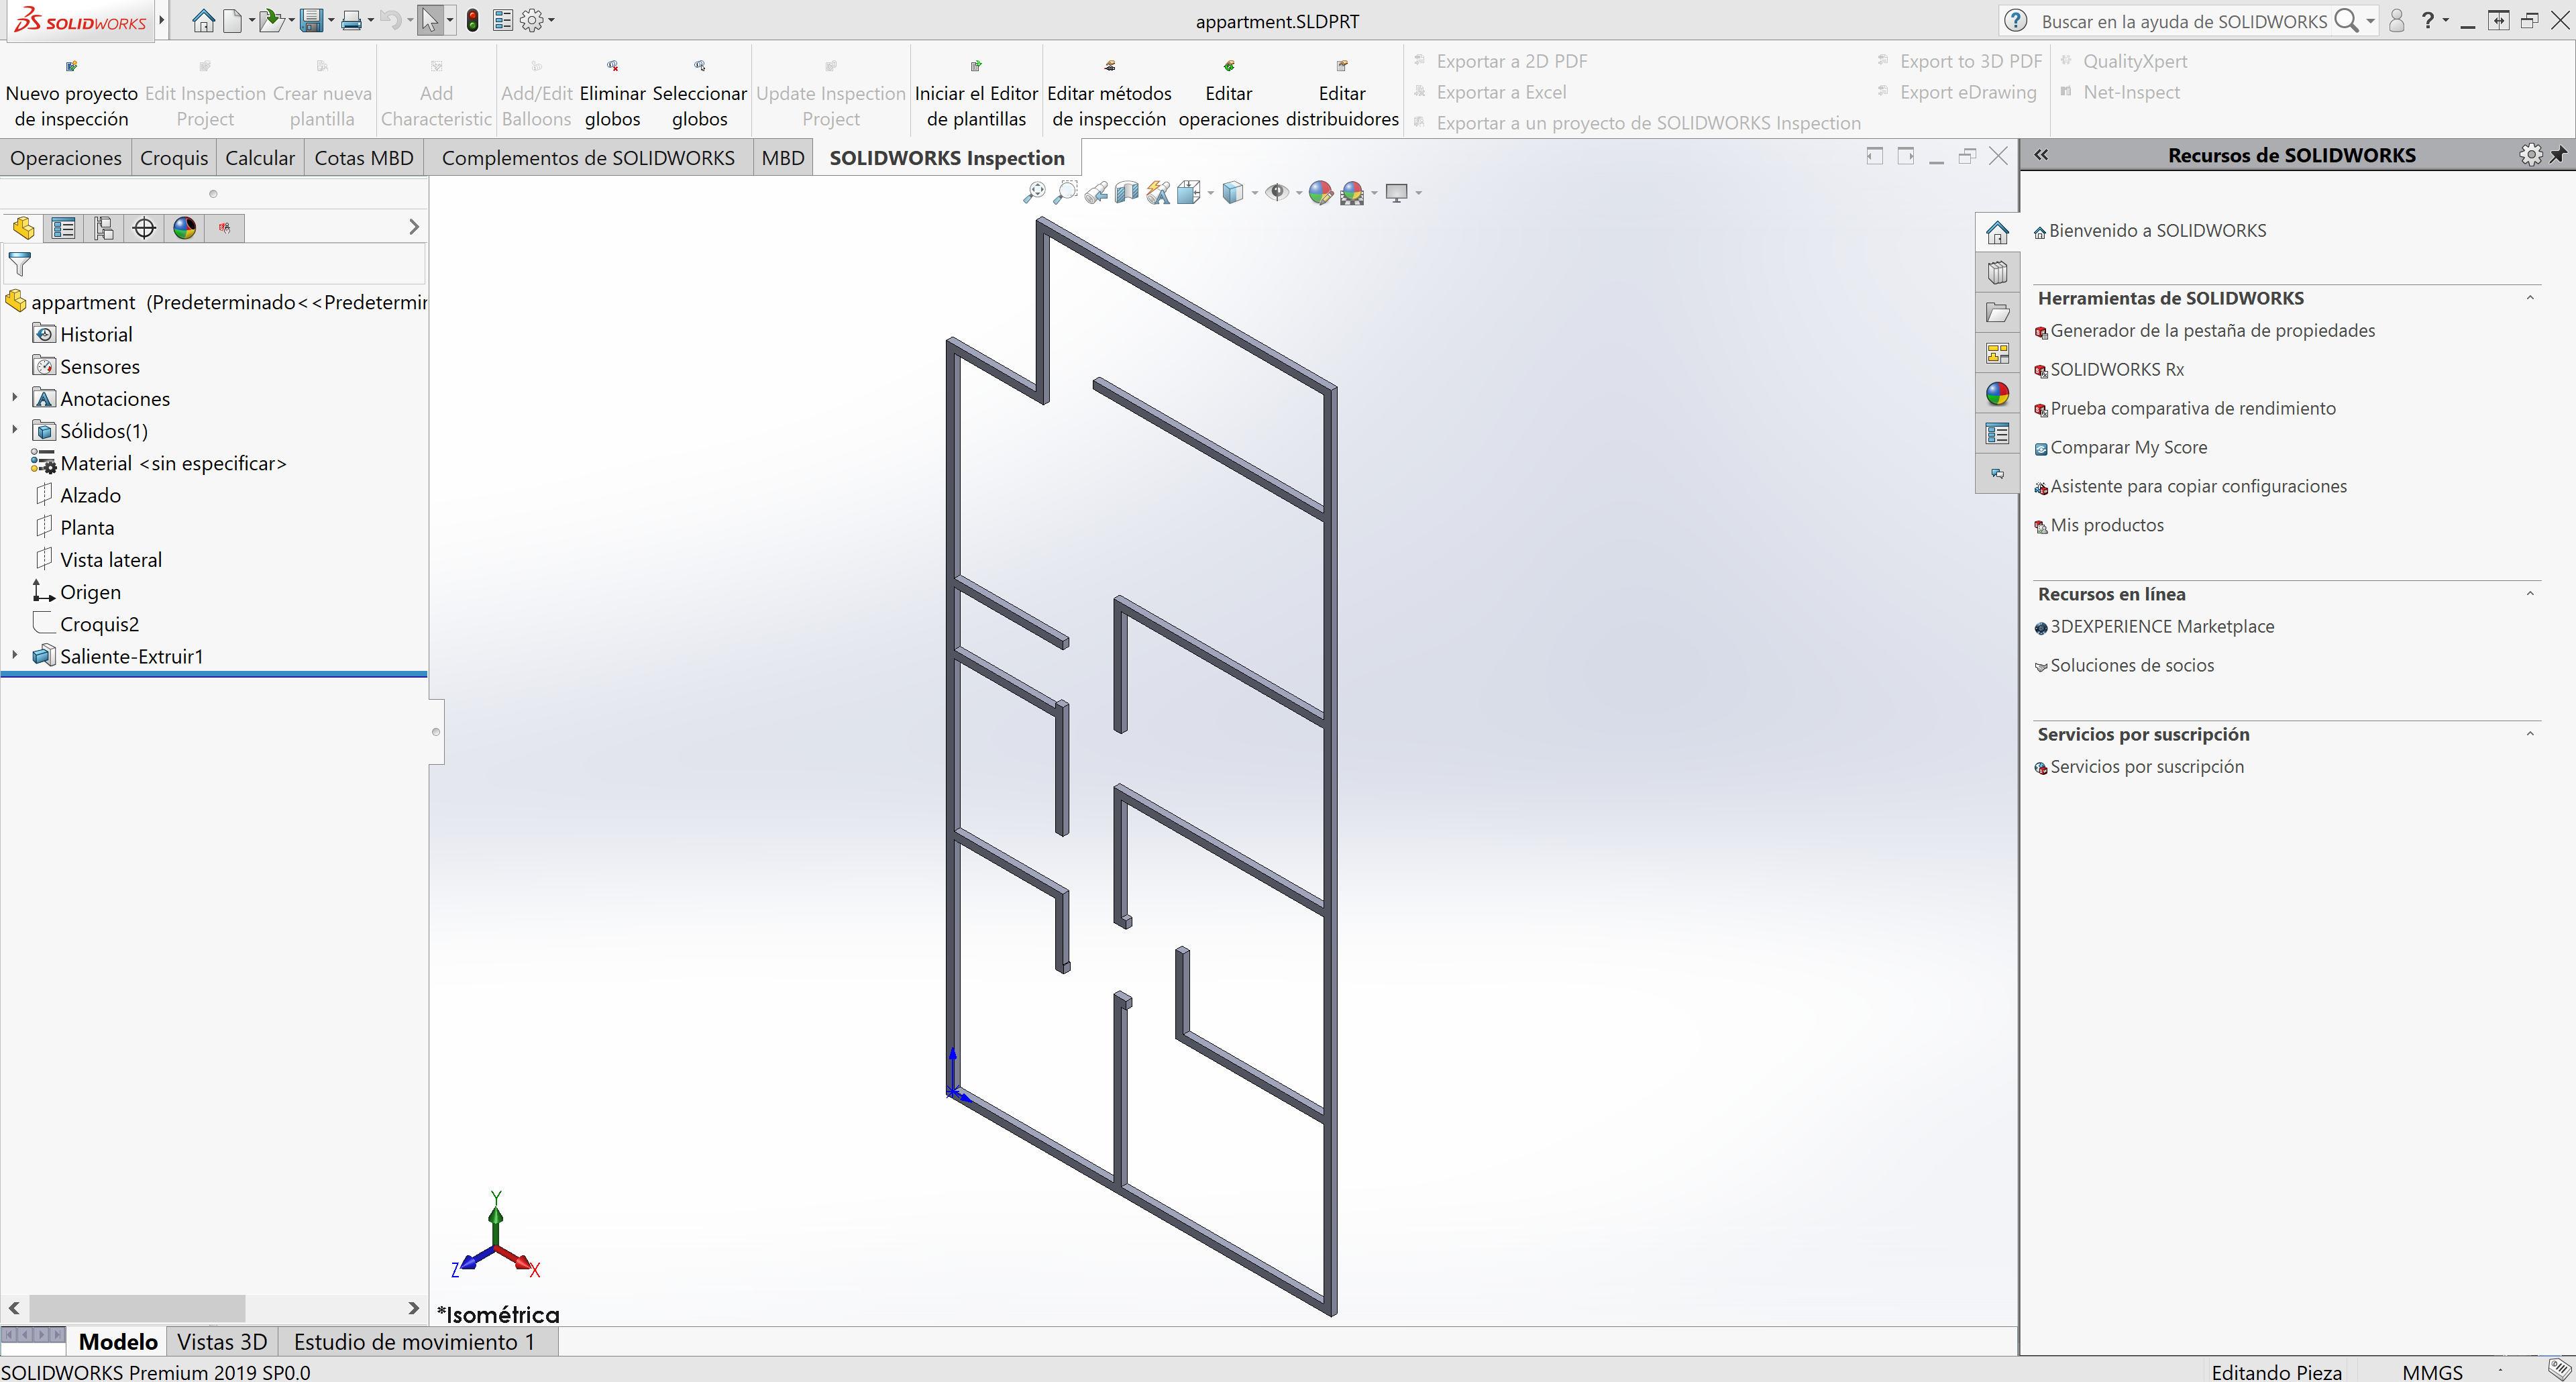
\includegraphics[width=0.75\linewidth, keepaspectratio]{mapa_solidworks}
  \caption{Mapa tridimensional del mapa del sitio a navegar hecho en SolidWorks.}
  \label{fig:mapa_solidworks}
\end{figure}

\begin{figure}[ht!]
  \centering
  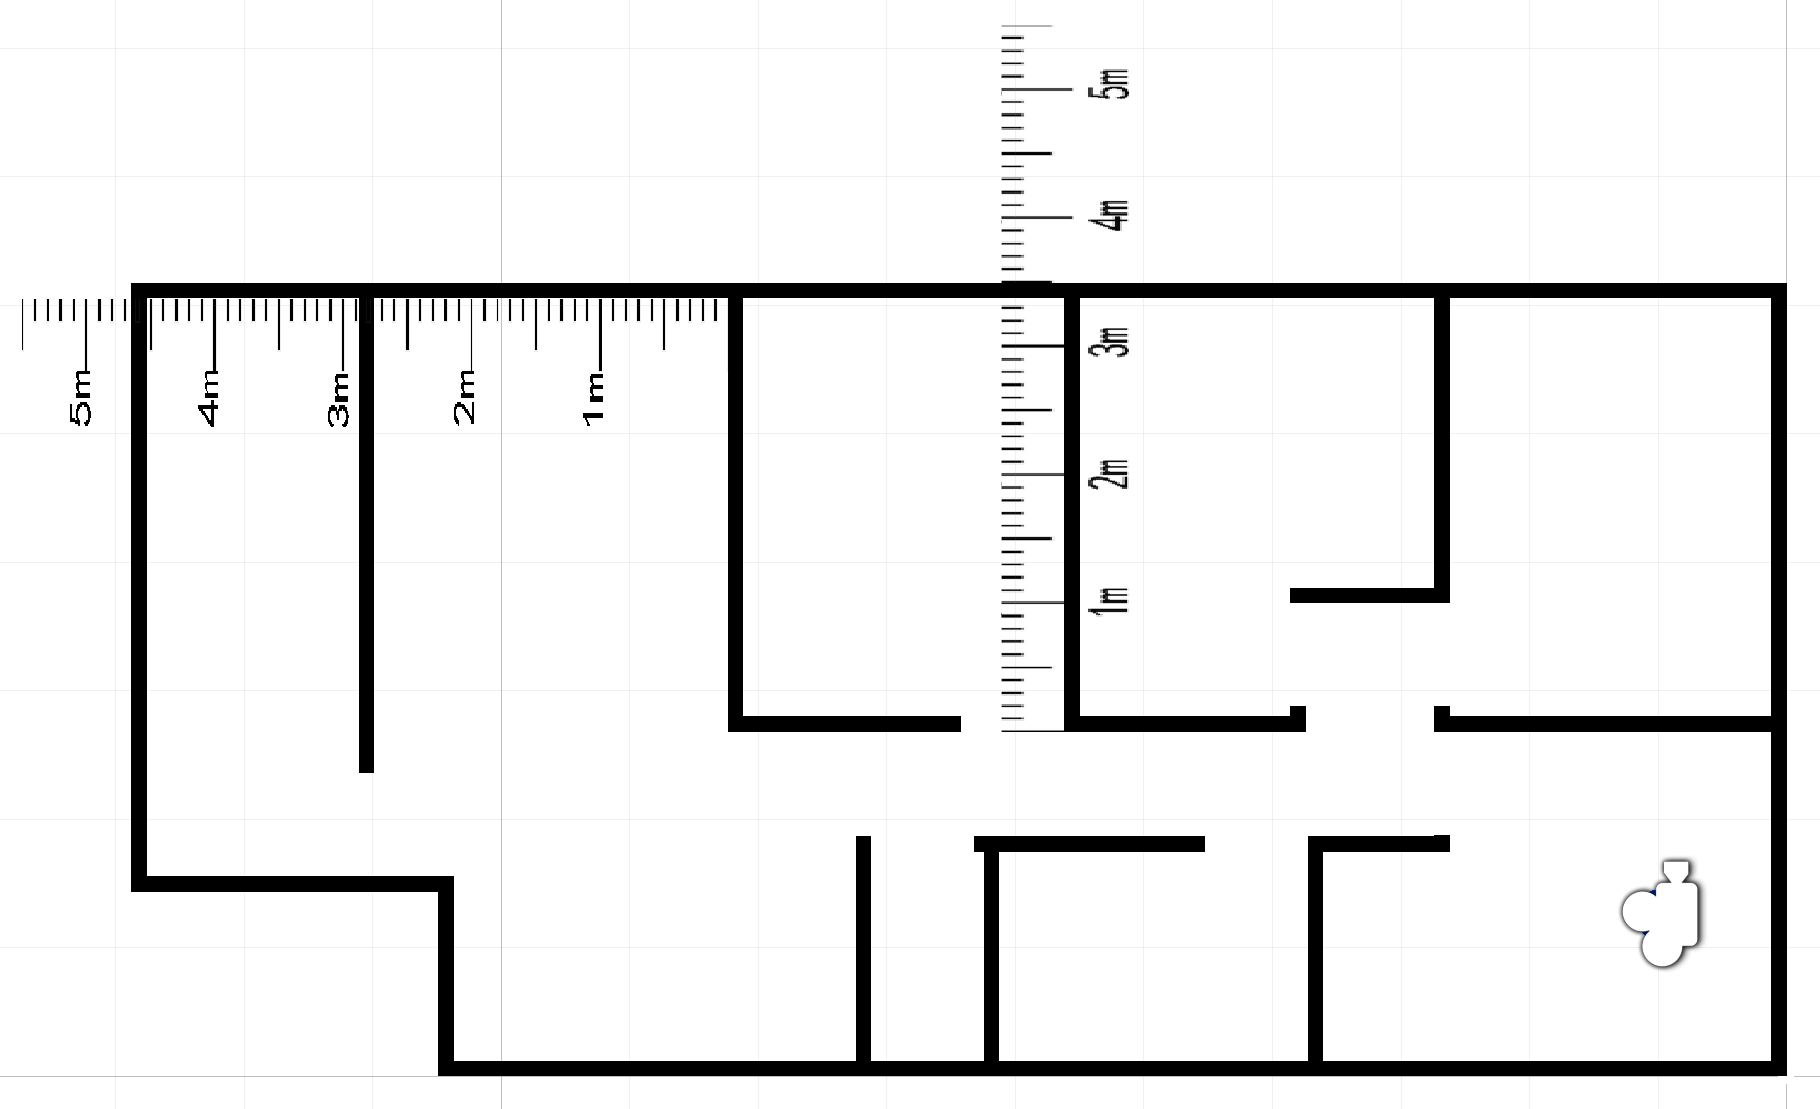
\includegraphics[width=0.65\linewidth, keepaspectratio]{escala_mapa}
  \caption{Uso de \textit{zzz Ruler} para asegurar la correcta escala del mapa en Unity.}
  \label{fig:escala_mapa}
\end{figure}

Para representar el usuario, referido como \textit{Player}, se inserta un cilindro en la escena.
Se añade también un \textit{prefab} de una flecha encima del cilindro para indicar la orientación del usuario y un cubo invisible por delante del cilindro para utilizarlo en cálculos auxiliares que se explicarán más adelante.
Se crea una cámara como hijo del cilindro que apunta hacia éste desde arriba para capturar su movimiento en el mapa.
Se crea una \textit{Render Texture} en la carpeta \textit{/Textures} del proyecto.
En la propiedad \textit{Target Texture} de la cámara mencionada, se selecciona la textura creada para poder usarla luego en un minimapa mostrado en la interfaz gráfica de la aplicación.

Se crea un script y se lo asocia al objeto \textit{Player Controller} para controlar el movimiento del cilindro para que corresponda al movimiento real del usuario.
El \cref{lis:player_controller} muestra el código implementado.
Se puede apreciar que \textit{Frame.Pose} contiene la posición y orientación dadas por ARCore relativas al punto inicial.
Estos datos relativos se traducen a una posición y orientación absoluta en el mapa gracias a la calibración por códigos QR.

\lstinputlisting[language = {[Sharp]C}, caption = {Código para el seguimiento de movimiento}, label = {lis:player_controller}]{../external/player_controller.cs}

\FloatBarrier

\subsection{Calibración}

Al iniciar la aplicación, antes de poder comenzar a navegar, el usuario debe escanear un código QR correspondiente a un punto de referencia del mapa.
Estos códigos contienen simplemente el nombre del punto de referencia y son creados y colocados en el sitio a navegar con antelación.

Los puntos de referencia son objetos vacíos en Unity cuyo nombre se usa para identificarlos, las componentes \textit{x} y \textit{z} de su posición reflejan la ubicación en el mapa y la rotación alrededor del eje \textit{y}, la orientación.

El objeto \textit{QR Scanner} contiene el script que maneja la calibración.
Como muestra el \cref{lis:qr_scan}, en cada fotograma, el lector de ZXing busca un código QR en la imagen de la cámara, cuando encuentra uno, se analiza el contenido del código y, si coincide con un punto de referencia, se procede con la reubicación.

\lstinputlisting[language = {[Sharp]C}, caption = {Código para la lectura de códigos QR}, label = {lis:qr_scan}]{../external/qr_scan.cs}

La reubicación, mostrada en \cref{lis:relocate_calib}, consiste en trasladar el cilindro que representa al usuario hasta la posición del punto de referencia y en calcular la diferencia en la orientación que luego se ajustará en el script de seguimiento de navegación como pudo verse en \cref{lis:player_controller}.
Cabe resaltar que no se utilizó la siguiente línea

\lstinline[language = {[Sharp]C}]{player.transform.position = child.position;}

\noindent porque el componente \textit{NavMeshAgent} que posee el usuario no permite el movimiento cuando entre la posición anterior y actual hay una pared.
Se utiliza en cambio la función \lstinline{Warp()} de dicho componente \textit{NavMeshAgent}.

\lstinputlisting[language = {[Sharp]C}, caption = {Código para la reubicación del usuario en el mapa}, label = {lis:relocate_calib}]{../external/relocate_calib.cs}

\subsection{Navegación}

La interfaz de usuario contiene un objeto \textit{Dropdown}, o menú desplegable, en el que se enumeran los puntos de referencia.
Cuando el usuario selecciona uno de estos puntos, el \textit{Listener} del evento \textit{onValueChanged} del menú se activa y llama a la función \lstinline{SetTargetDestination()}, ver \cref{lis:setTargetDestination}, que establece la posición objetivo y activa y posiciona los colisionadores para poder ubicar la flecha y el pin en realidad aumentada.
% El colisionador de la flecha se coloca en la posición actual del usuario y el del pin en la posición deseada.

\lstinputlisting[language = {[Sharp]C}, caption = {Código que se ejecuta al seleccionar un punto de referencia del menú desplegable}, label = {lis:setTargetDestination}]{../external/setTargetDestination.cs}

\subsubsection{Navegación en minimapa}

Para implementar esta funcionalidad se siguió \href{https://learn.unity.com/tutorial/unity-navmesh}{el siguiente tutorial} \cite{navMesh} que explica cómo utilizar los distintos componentes y funciones de NavMesh.

Una vez seleccionada la ubicación de destino, el \cref{lis:calculatePath} muestra cómo se calcula constantemente el camino entre la posición actual del usuario y la posición deseada teniendo en cuenta los obstáculos en el mapa con la función \lstinline{CalculatePath()} de NavMesh y cómo se representa dicho camino en el minimapa utilizando el componente \textit{LineRenderer}.
Este código es parte del script del objeto \textit{Path Finder}.

\lstinputlisting[language = {[Sharp]C}, caption = {Código para el cálculo del camino y su representación gráfica}, label = {lis:calculatePath}]{../external/calculatePath.cs}

Se agrega un objeto con el componente \textit{NavMeshSurface}.
La \cref{fig:navmeshsurface} muestra las configuraciones realizadas.
Al hacer click en \textit{Bake}, se genera la superficie navegable.

\begin{figure}[ht!]
  \centering
  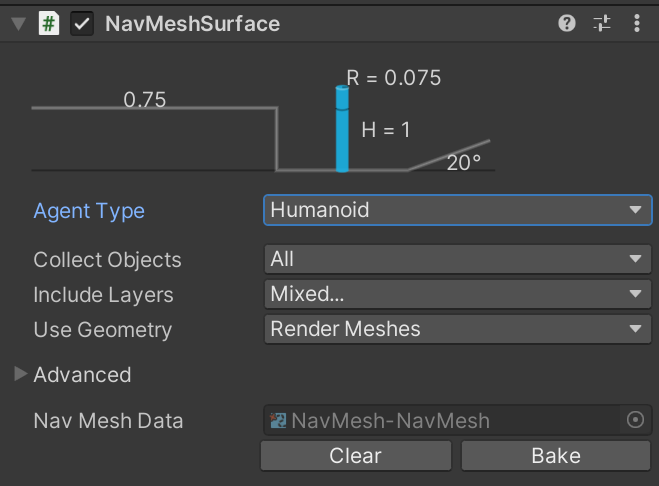
\includegraphics[width=0.45\linewidth, keepaspectratio]{navmeshsurface}
  \caption{Configuraciones de \textit{NavMeshSurface}.}
  \label{fig:navmeshsurface}
\end{figure}

Para que NavMesh reconozca las paredes como obstáculos a evitar, es necesario agregar el componente \textit{NavMeshModifier} al mapa.
En sus opciones, activar \textit{Override Area} y seleccionar \textit{Not Walkable} en \textit{Area Type}.
De esta manera, Navmesh sabrá que el agente no puede caminar por las paredes.
Después de esto, es necesario hacer click en \textit{Bake} nuevamente para que se reflejen los cambios.

Al objeto \textit{Player} se le añade un componente \textit{NavMeshAgent}.
Por defecto, este componente se desactiva y el usuario puede moverse incluso fuera de las zonas caminables de NavMesh.
Esto quiere decir que el usuario podría ``atravesar paredes'' por ejemplo.
Esto es útil porque el seguimiento de navegación presenta, como se explicó anteriormente, errores acumulativos y, en lugares como pasillos angostos, el usuario podría ``quedarse atrapado'' en habitaciones en las que realmente no se encuentra.
Si, aún así, se quiere que el usuario no pueda atravesar paredes, se activa entonces este componente.
La opción para activar o desactivar el colisionado con paredes está incorporado en el menú de configuraciones de la interfaz de usuario.

\subsubsection{Navegación en realidad aumentada}

Además de las indicaciones en el minimapa, se agregan indicaciones en realidad aumentada.
Se coloca una flecha en frente del usuario indicando la dirección a seguir durante la navegación y cuando llega a destino, se coloca un pin.
Estos objetos se fijan en un punto del entorno físico de manera tal que, al moverse el usuario, los objetos quedan anclados a ese punto.
De esta manera, el efecto de realidad aumentada es más inmersivo.

Para ello, primero se crean dos objetos con colisionadores del tipo \textit{Capsule Collider}, uno para la flecha y otro para el pin.
Al colisionador de la flecha se lo fija en la posición del usuario en un instante dado.
Cuando la colisión entre el usuario y este colisionador se activa, se coloca frente al usuario una flecha.
El dirección de la flecha se calcula como el ángulo entre la dirección en la que el usuario está mirando (representado por la recta que une el usuario y el cubo auxiliar) y la dirección en la que se encuentra el próximo punto del camino calculado (recta que une el usuario y el segundo punto del objeto \textit{LineRenderer}, siendo el primer punto el correspondiente a la posición del usuario).

El script \textit{ArrowPlacer}, mostrado en parte en el \cref{lis:arrowPlacer}, se lo añade al objeto usuario, \textit{Player}, ya que las colisiones que se buscan son entre \textit{Player} y el colisionador de la flecha y \textit{Player} y el colisionador del pin y las funciones utilizadas \lstinline{OnTriggerEnter(Collider)} y \lstinline{OnTriggerExit(Collider)} son llamadas cuando el objeto que contiene el script entra o sale de una colisión y tienen como argumento al colisionador con el que dicho objeto interactuó.

Cada vez que el usuario sale del volumen del colisionador de la flecha, la flecha actual se elimina y se crea una nueva enfrente del usuario hasta que éste entre en contacto con el colisionador del pin ubicado en la posición deseada.
La flecha se elimina y se coloca el pin.
Si el usuario sale del volumen del colisionador del pin, entrará nuevamente en el colisionador de la flecha.

\lstinputlisting[language = {[Sharp]C}, caption = {Código para el manejo de elementos de realidad aumentada}, label = {lis:arrowPlacer}]{../external/arrowPlacer.cs}

\subsubsection{Navegación por indicaciones de voz}

Para complementar las instrucciones de navegación visuales, se añaden además instrucciones sonoras.
En primer lugar, se crean los archivos de sonido con una herramienta de texto-a-voz, como por ejemplo \href{https://notevibes.com/}{Notevibes}.
Las instrucciones de voz generadas son ``Gire a la derecha'', ``Gire a la izquierda'', ``Continúe derecho' y ``Ha llegado a destino''.

Siguiendo el \href{https://www.youtube.com/watch?v=6OT43pvUyfY}{siguiente tutorial} \cite{sound}, se puede añadir audio a una aplicación de Unity.
Se crea una clase \textit{Sound} para albergar el archivo, nombre y propiedades como volumen y tono de cada sonido.
Luego, se crea un objeto \textit{Audio Manager} con un script para controlar la reproducción de sonido en la aplicación al que se le asocian los objetos \textit{Sound} desde el inspector como muestra la \cref{fig:audio_manager}.

\begin{figure}[ht!]
  \centering
  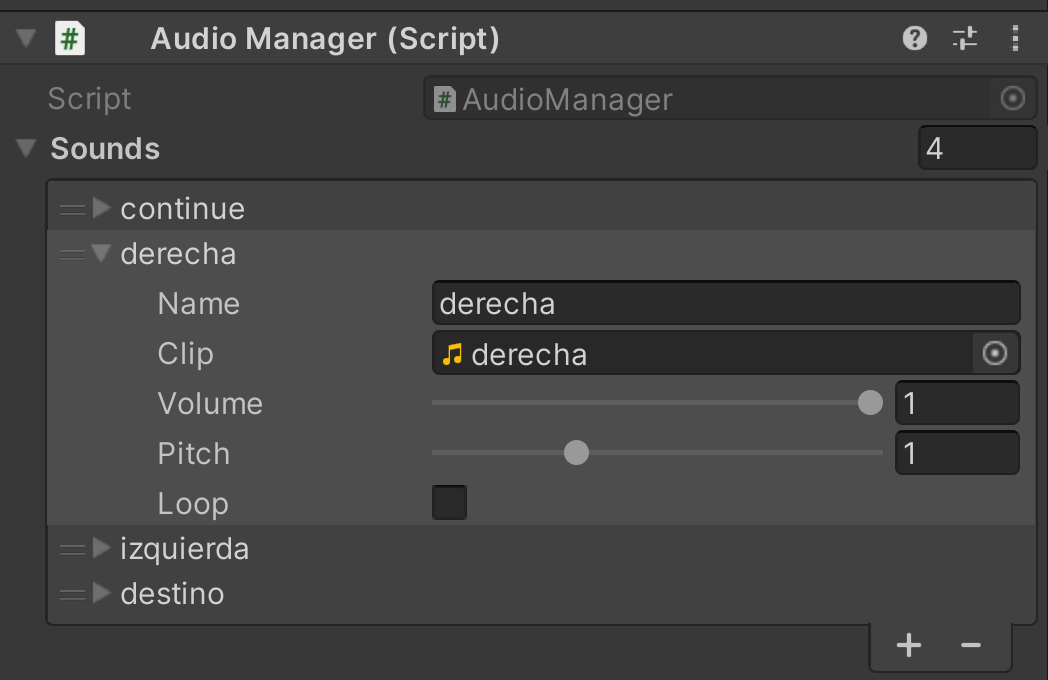
\includegraphics[width=0.55\linewidth, keepaspectratio]{audio_manager}
  \caption{\textit{Audio Manager} en el inspector de Unity.}
  \label{fig:audio_manager}
\end{figure}

El \cref{lis:audioManager} describe la función de \textit{Audio Manager} a la que se llama para reproducir audio.
Se utiliza una corrutina para esperar hasta que cualquier otra pista de audio termine de reproducirse para poder reproducir una nueva, de esta manera, se evita que se superpongan.

\lstinputlisting[language = {[Sharp]C}, caption = {Código para manejar la reproducción de audio.}, label = {lis:audioManager}]{../external/audioManager.cs}

Se añade el código en \cref{lis:arrowPlacerAudio} al scrip de \textit{ArrowPlacer} descripto previamente.
Cuando se crea una nueva flecha, se utiliza el ángulo calculado para determinar cuál instrucción reproducir.
Se compara con el ángulo de la flecha anterior para no estar constantemente repitiendo el mismo comando y sólo reproducir la instrucción cuando ésta sea la primera o bien distinta de la anterior.
Cuando se llega a destino y se coloca el objeto pin, se reproduce también la indicación correspondiente.

\lstinputlisting[language = {[Sharp]C}, caption = {Código agregado a \textit{ArrowPlacer} para reproducir la indicación de voz según la flecha o pin que aparece en pantalla.}, label = {lis:arrowPlacerAudio}]{../external/arrowPlacerAudio.cs}

\subsection{Descarga de datos}

\subsubsection{Servidor en Raspberry Pi}

Para el script del server, se usa como plantilla el ejemplo \textit{rfcomm-server.py} de PyBluez \cite{pybluez}.
El script modificado para adaptarla a esta aplicación se puede ver en \cref{lis:bt_server}.
Puede observarse en el script que, para crear la comunicación RFCOMM, es necesario indicar un UUID (\textit{Universally Unique Identifier}) que es un número de 128 bits que identifica un servicio particular provisto por un dispositivo Bluetooth.
Para esta comunicación se usa el servicio \textit{Generic Attribute Profile} (GATT) que provee las bases para la transferencia bidireccional de pequeños fragmentos de datos para aplicaciones de bajo consumo.
Para encontrar el UUID del servicio GATT de la Raspberry Pi, se ejecuta el siguiente comando en consola y se busca la línea \lstinline{UUID: Generic Attribute Profile (#UUID)}.

\noindent\begin{minipage}{\linewidth}
\begin{lstlisting}
$ bluetoothctl
# show
\end{lstlisting}
\end{minipage}

Se añade un bucle para reintentar la conexión cuando esta falla.
Una vez establecida la conexión, se espera a que el cliente comience la comunicación.
Cuando se recibe un \textit{``Hello''}, se envía al cliente la lista de puntos de referencia codificados como \lstinline{[<<nombre>>;<<posición en x>>;<<posición en z>>;<<rotación en y>>]}.
Al final del mensaje se envía \textit{``Done''} para indicarle al cliente que ha finalizado la comunicación.

Se guarda el script, se lo hace ejecutable

\noindent\begin{minipage}{\linewidth}
\begin{lstlisting}
$ chmod +x bt_server.py
\end{lstlisting}
\end{minipage}

\noindent y se configura para que se ejecute automáticamente en el arranque del sistema.

\lstinputlisting[language = {Python}, caption = {Código para el servidor en la comunicación Bluetooth}, label = {lis:bt_server}]{../external/bt_server.py}

\subsubsection{Cliente en teléfono}

El objeto \textit{Map Download Menu} contiene un script que se encarga de la lógica detrás de los eventos vinculados con los elementos gráficos del menú para la descarga de los datos de navegación así como también de implementar las funciones para el cliente de la comunicación Bluetooth.
El \cref{lis:bt_client} muestra las funciones para la lectura y el envío de mensajes con el servidor usando como base el ejemplo \textit{Bluetooth Terminal} del plugin \textit{Android \& Microcontrollers / Bluetooth}.
Puede verse que los datos recibidos se almacenan en \lstinline{_processText.text} tanto para mostrar en la interfaz de usuario, como para procesar los datos recibidos internamente.

\lstinputlisting[language = {[Sharp]C}, caption = {Código para el cliente en la comunicación Bluetooth}, label = {lis:bt_client}]{../external/bt_client.cs}

El \cref{lis:mapDownload} muestra cómo se establece la comunicación cliente-servidor y cómo se tratan los datos recibidos para incorporarlos al mapeado.
Como se explicó anteriormente, luego de establecer la conexión, el cliente envía el mensaje \textit{``Hello''} y espera hasta recibir \textit{``Done''}.
Se eliminan los puntos de referencia existentes en caso de que ya se hayan descargados otros datos previamente.
Se decodifica el mensaje usando \textit{Regex}, expresiones regulares, para comprobar si una cadena de caracteres se corresponde con un patrón.
De esta manera, se identifican los puntos de referencia individualmente separados por paréntesis y, para cada uno, el nombre y coordenadas separados por puntos y comas.
Luego, se crea un objeto para cada punto de referencia como hijo de un objeto \textit{parent} que los agrupa a todos y se modifican sus propiedades con los datos decodificados.
Se crean también etiquetas para mostrarse en el punto correspondiente del minimapa con los nombres de los puntos de referencia utilizando el paquete TextMeshPro incluido en Unity que permite manejar texto con una gran flexibilidad.

\lstinputlisting[language = {[Sharp]C}, caption = {Código para la decodificación de datos recibidos y añadido de los puntos de referencia}, label = {lis:mapDownload}]{../external/mapDownload.cs}

\subsection{Interfaz de usuario}

Para la interfaz de usuario que se muestra en la pantalla del teléfono, se crea un objeto \textit{Canvas} en donde se colocan todos los objetos gráficos.
En la interfaz principal, \cref{fig:ui_main}, hay un menú desplegable en la esquina superior izquierda con los puntos de referencia para elegir el destino, el minimapa en la esquina inferior izquierda, un botón para el menú de configuraciones en la esquina superior derecha y, en el centro, una etiqueta de texto para mostrar mensajes al usuario.

\begin{figure}[ht!]
\centering
\begin{subfigure}[b]{0.70\textwidth}
   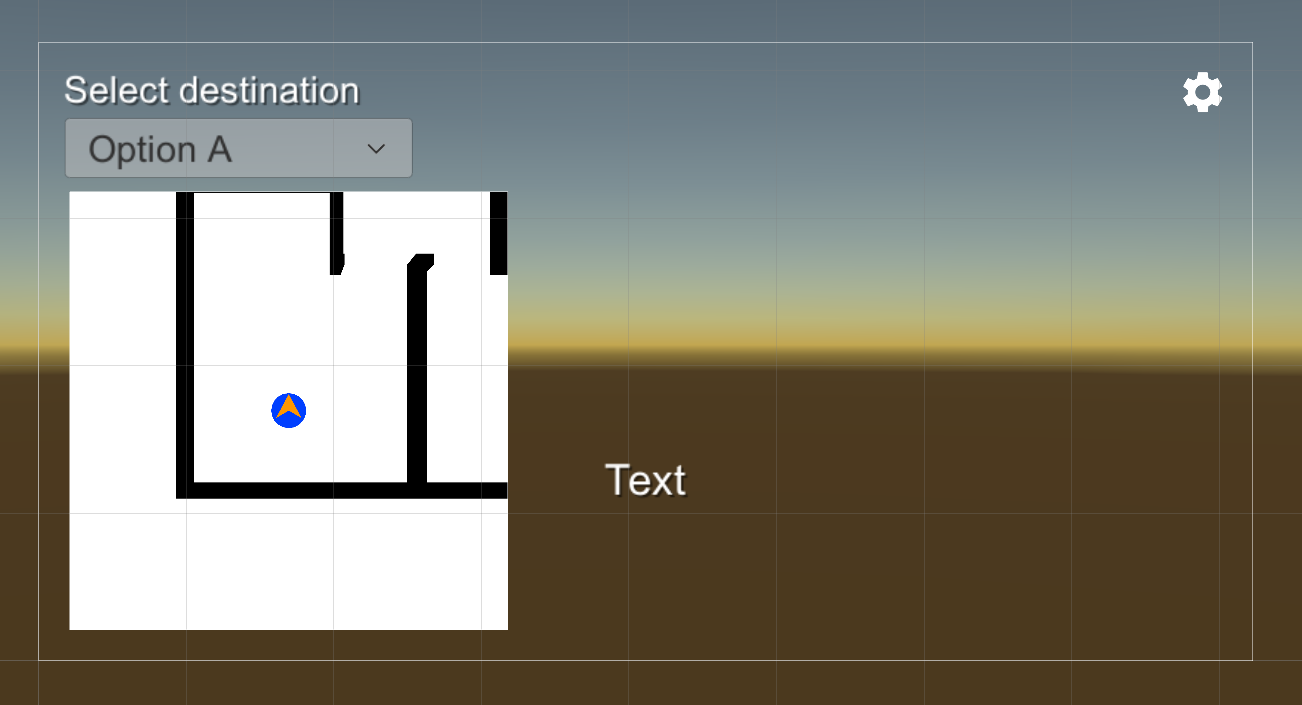
\includegraphics[width=1\linewidth,keepaspectratio]{ui_main}
   \caption{Pantalla principal.}
   \label{fig:ui_main}
\end{subfigure}
\vspace{1em}

\begin{subfigure}[b]{0.70\textwidth}
   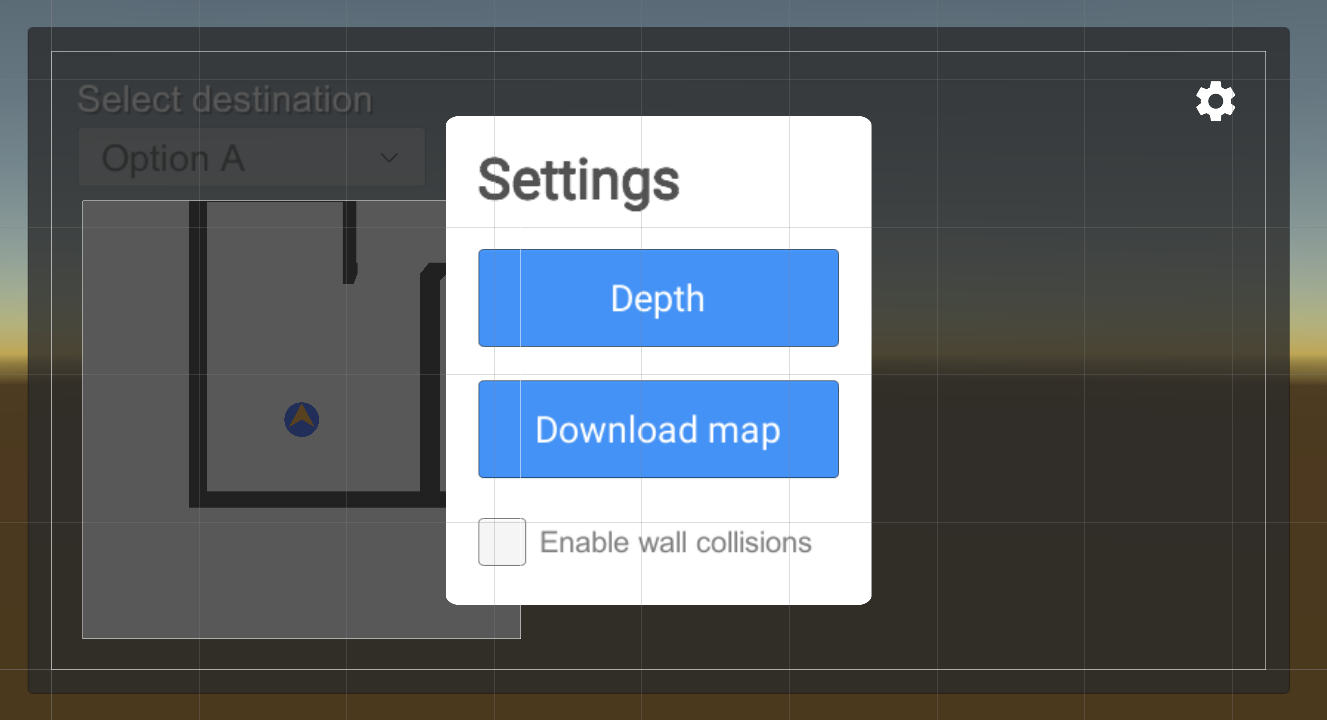
\includegraphics[width=1\linewidth,keepaspectratio]{ui_menu}
   \caption{Menú de configuraciones.}
   \label{fig:ui_menu}
\end{subfigure}
\vspace{1em}

\begin{subfigure}[b]{0.70\textwidth}
   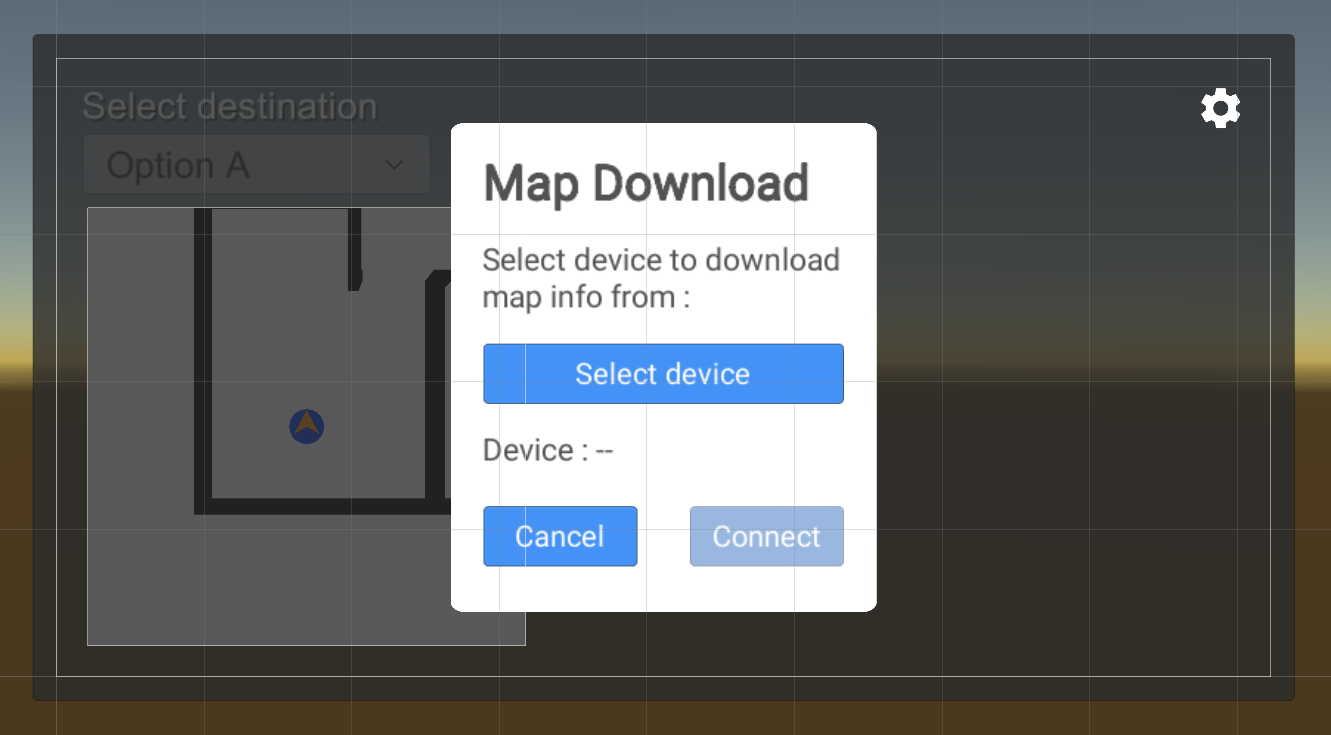
\includegraphics[width=1\linewidth,keepaspectratio]{ui_map_download}
   \caption{Menú para descarga de datos del mapa.}
   \label{fig:ui_map_download}
\end{subfigure}
\vspace{1em}

\caption{Interfaz gráfica de la aplicación para el teléfono.}
\end{figure}

El minimapa es un objeto con el componente \textit{Raw Image}.
En la propiedad \textit{Texture}, se selecciona la textura creada por la cámara que sigue al cilindro que representa al usuario.
Para aprender más sobre minimapas, ver \href{https://www.youtube.com/watch?v=28JTTXqMvOU}{el siguiente tutorial} \cite{miniMap}.
Se añade un script basado en \cite{indoorNavRacoons} para permitir controlar la cámara según gestos con los dedos en la pantalla táctil.
Moviendo un dedo por la pantalla, la cámara se mueve en el sentido contrario.
Al elegir una opción del menú desplegable, el usuario realiza ese mismo movimiento, por lo que se debe detectar cuando el menú está desplegado y no mover la cámara.
Con dos dedos, se puede acercar o alejar la cámara del usuario modificando su campo de visión, \textit{field of view}.
Con dos toques rápidos, la cámara vuelve a su estado inicial.

Al tocar el botón de configuraciones, se abre el menú mostrado en \cref{fig:ui_menu}.
El botón \textit{Depth} abre el menú ya presente en la plantilla \textit{HelloAR} que permite activar o desactivar opciones de profundidad para realidad aumentada de modo que si el objeto virtual está ubicado detrás de un objeto real, se oculta la parte tapada para aumentar la inmersión de la experiencia.
Se deja esta opción, sin embargo no es relevante para esta aplicación.
El botón \textit{Download map} abre el menú que se ve en \cref{fig:ui_map_download}.
Hay un botón que abre la interfaz de Android para seleccionar un dispositivo Bluetooth.
Una vez seleccionado, se habilita el botón \textit{Connect} que intentará establecer conexión con el dispositivo y obtener los puntos de referencia.

\end{standalone}
\end{document}
